\documentclass[10pt,twocolumn]{article}

% use the oxycomps style file
\usepackage{oxycomps}

% usage: \fixme[comments describing issue]{text to be fixed}
% define \fixme as not doing anything special
\newcommand{\fixme}[2][]{#2}
% overwrite it so it shows up as red
\renewcommand{\fixme}[2][]{\textcolor{red}{#2}}
% overwrite it again so related text shows as footnotes
%\renewcommand{\fixme}[2][]{\textcolor{red}{#2\footnote{#1}}}

% read references.bib for the bibtex data
\bibliography{references}

% include metadata in the generated pdf file
\pdfinfo{
    /Title (Password Manager: Secure Digital Access Through Password Management and User-Centric Security Education)
    /Author (Jadriel Delim)
}

% set the title and author information
\title{Password Manager: Secure Digital Access Through Password Management and User-Centric Security Education}
\author{Jadriel Delim}
\affiliation{Occidental College}
\email{jdelim@oxy.edu}

\begin{document}

\maketitle


\section{Introduction and Problem Context}
% This section should motivate why the project is interesting both to you and to the computer science community or the general public.
% You should also justify the difficult of the project.
% As a rough guideline, your project should be either narrow but deep in a subfield of CS, or broadly reaching across subfields without being too shallow.
% It should be comparable to the amount of work/content in an upper-level elective.
Password managers are necessary in the modern age of the internet due to the numerous usernames and passwords people have for a variety of websites and applications. Most people don't realize the importance of having strong passwords and have resorted to ``choosing simple passwords and reusing them across sites" \cite{li2014emperor}. In fact, the reason why non-users of password managers hesitate to use them are due to security concerns, mostly because of a lack of understanding of how password managers work \cite{fagan_albayram_khan_buck_2017}. There is a fear non-users express that the vault containing all their passwords can easily be hacked. However, there are many layers of encryption and security to prevent that from happening, granted that they utilize a strong and secure master password. If you look at online forums such as Reddit, there are more reports of users being locked out of their vaults because they forgot their passwords compared to being hacked. On the other hand, users of password managers often point to the convenience and usefulness of utilizing a password manager, rather than the security aspect\cite{fagan_albayram_khan_buck_2017}. For instance, some password managers can auto-fill passwords, generate passwords for new accounts, and conveniently store credentials in their own designated folder. Thus, this project will not only incorporate the main features of a password manager, but also aim to help users understand the security and necessity behind password managers.
\paragraph{}
Additionally, there is also a personal aspect to this project as my dad had his Facebook hacked a couple years ago and had not been able to recover it since. This was because he had an old and unused email attached to his account which was most likely hacked due to the use of a weak password. This situation not only caused a lot of stress for him, but also was time-consuming as he tried to contact customer service and had to change passwords for his emails and bank accounts out of an abundance of caution. If he had utilized a password manager with a strong master password, this situation would likely not have happened. Overall, I want to not only study and learn more about the encryption and security behind password managers, but also spread awareness about the necessity of having a password managers to give people peace of mind when, not if, an unknown actor tries to access their credentials.


\section{Technical Background}

% This section introduces the technical knowledge necessary to understand your project, including any terminology and algorithms.
% You should assume that the reader is a CS undergraduate like yourself, but not necessarily familiar with AI/ML/HCI/apps/video games/etc.

\subsection{Brief Technical Overview}
Before getting into the technical aspect, there are 3 essential things to understand in regards to password manager security: encryption, hashing, and salting. Most people often confuse one for the other, so clarification here is needed. Encryption involves scrambling information where only someone else with the corresponding key can unscramble and read the information. This is a two-way function because something that is encrypted can be decrypted. Hashing involves a hashing algorithm where it maps data of any  size to a fixed length known as a hash value. For example, the hashing algorithm SHA-256 outputs a hash value of 256 bits. A hash cannot be reverse-hashed, and each hash value is unique. Salting involves adding a unique value to the end of a password as to create a different hash value and adds a layer of security. It is important that the salt for each password should be different, so that two users with the same password doesn't show the same hash value.

\subsection{Architecture}
Now that we understand the fundamentals, my password manager will try to adhere to the National Institute of Standards and Technology (NIST) standards as much as possible \cite{grassi_fenton_newton_perlner_regenscheid_burr_richer}. This means having a set of requirements when users create their master passwords. Users cannot have ``passwords obtained from previous breach corpuses, dictionary words, repetitive or sequential characters, or context-specific words" \cite{grassi_fenton_newton_perlner_regenscheid_burr_richer}. Additionally, part of the password verification process includes assisting the user in choosing a strong master password. This might look like including a password strength meter so that users can visually see the strength of their password or simply a list of requirements telling the user which aspects of a strong password they are missing.

\paragraph{}
To continue, the cryptography architecture will look something like the following. The password manager is able to encrypt/decrypt the credential database ``using a key derivation function starting a user provided secret" \cite{li2014emperor} which is the user's master password. This derivation function is a one-way cryptographic function meaning that it is computationally infeasible to reverse the hash and obtain the original master password. However, this derived key will not be used to encrypt the database, but rather a random symmetric key. This way, if the user changes their password, there will be no need to re-encrypt the entire database. The key will just be derived again with the new password, and then encrypt the symmetric key with the newly generated key. Here is a numbered list outlining the encryption process:
\begin{enumerate}
    \item User types their password (PASS): \textcolor{blue}{\textbf{AmazingPassword1289863}}
    \item Use a key derivation function (PBKDF2) to generate a key (DKEY) using PASS: \textcolor{blue}{\textbf{8d6x82..ahfhwhw6}}
    \item Generate a random key (RKEY): \textcolor{blue}{\textbf{sh872h08xj...827hsuz8}}
    \item Encrypt RKEY with DKEY and store the encrypted key (EKEY): \textcolor{blue}{\textbf{snnxaiu82190...2gshx868}}
\end{enumerate}
The encrypted key is stored (EKEY) and cannot be derived back to the RKEY, DKEY, or PASS. Only EKEY is stored, nothing else. When the user unlocks the database, they type in their PASS, then DKEY is derived from it, and EKEY is decrypted using DKEY, getting RKEY to decrypt the database through symmetric encryption. If the user intends to change their password, the process might look like the following:
\begin{enumerate}
    \item User enters their current password (CURRPASS)
    \item DKEY is derived, decrypt EKEY, which retrieves RKEY on plaintext
    \item Ask for a new password (NEWPASS)
    \item Derive the new DKEY2 from NEWPASS
    \item Encrypt RKEY with DKEY2 which creates EKEY2
    \item Store EKEY2
\end{enumerate}

\paragraph{}
Lastly, I will be using Python as my programming language, a PostgreSQL database, and a command line interface (CLI) for the user interaction. While a CLI might not look as neat or fancy as an application interface, it still allows me to implement the features I want to include as well as putting more focus on the encryption aspect of the project. The overall focus of the project can be divided into three parts: the encryption, database, and educational process.
\subsection{Exploring Encryption and Hashing Algorithms}
The main part of this project has to do with the implementation of my cryptographic architecture. Part of this implementation involves choosing the best and most appropriate encryption and hashing algorithms to ensure user security while also maintaining efficiency. Let's explore how the key derivation function PBKDF2 and symmetric-key algorithm AES-256 works.
\paragraph{}
First, PBKDF2 is a key derivation function used to derive a secure key from a password or passphrase. It takes in an input password and a salt to produce a key of a certain specified length. This function is designed to be slow and computationally expensive. While the slowness and expensiveness initially seems to be a flaw, it actually makes it more resistant to brute-force or dictionary attacks which try to guess the password. PBKDF2 often uses a hash function, such as SHA-256, underneath to generate the key. SHA-256 is essentially just a hash function used to produce a fixed output, and is commonly used for digital signatures or data integrity checks. PKDF2 also allows for the configuration of the number of iterations which configures the time required to derive the key.
\paragraph{}
Next, AES-256 encryption uses a 256-bit key to encrypt and decrypt data and is classified as a symmetric-key encryption algorithm. Symmetric-key algorithms are essentially just a type of encryption algorithm that uses the same key for encrypting and decrypting. In AES-256, the information is first divided into 4x4 blocks of 16 bytes. Next, key expansion occurs where multiple round keys are recreated from the first key. The round key is then added to the data that has been subdivided into 4x4 blocks. Then, byte substitution occurs where each byte of data is substituted with another byte of data. Rows are then shifted in the 4x4 arrays, then a pre-established matrix mixes the 4x4 columns of the array. Finally, the AES algorithm repeats the round key addition step, then does the process all over again. This is a very brief and basic overview of the AES-256 encryption algorithm that is difficult to understand, but hopefully gives good insight into the security and complexity of the algorithm.

\section{Prior Work}
% This section describes of related and/or existing work.
% This could be scientific or scholarly, but may also be a survey of existing products/games.
% The goal of this section is to put your project in the context of what has already been done.
Finally, there are numerous password managers out there, some of the big names being LastPass, Dashlane, and Keeper password managers. These password managers not only do a good job in storing and securing personal information, but also offers features such as categorizing passwords and generating passwords \cite{alodhyani_theodorakopoulos_reinecke_2020}. This password manager will not be as complex as the well-known ones, but it should achieve an adequate amount of security as defined by NIST and other password manager guidelines. This project will be exclusively looking to password managers that utilize a master password as there are some password managers, such as MonoPass \cite{jeong_jung_2021}, that don't use a master password authentication.
\paragraph{}
Let's talk about potential vulnerabilities that password managers must take into account when designing their program. For instance, LastPass uses ``JavaScript to support all of its functionalities including the cryptographic operations", and also stores ``a user's websites credentials both locally to the user's machine and remotely to cloud storage servers" \cite{zhao2013security}. They use a variation of the password-based key derivation function PBKDF2, mentioned earlier in the Technical Background section. One of the vulnerabilities of LastPass ``lies in the insecure design of the master password remembering mechanism" \cite{zhao2013security}. This is because they actually store a user's master password into a local SQLite database table to allow the user to be automatically re-authenticated whenever they use LastPass again. Whether or not this master password is encrypted or not is irrelevant, as a ``locally saved master password, no matter encrypted or not, is vulnerable to local decryption attacks that can be performed by outsider attacks with the client-side stealing capability and/or the client-side computation capability" \cite{zhao2013security}. Connecting this back to the development of my password manager, it is crucial that the encrypted or decrypted versions of master passwords of users are never stored. Thus, this is why a randomly generated key (RKEY) for each user with no connection to the master password helps to prevent local decryption attacks.
\paragraph{}
When implementing my own password manager, I must take care in ensuring not only the responsible storing of users' credentials, but any other user information that may reveal information. This type of information might seem to be irrelevant, such as how many times a user has changed their master password, or websites that they have visited. However, the more information an attacker has on a user, the more likely they are to find information that can be used to access the user's database. 

\section{Methods}
% This section describes what exactly you will be working on.
% What are you building? How will it combine/incorporate ideas from the literature? Be specific about what you will be doing: talk about the specific algorithm you will implement/use, the specific dataset/platform/API, and what the outcome of your project will look like.
% All of these decisions should be justified as well.
\subsection{An Overall View}
There are essentially 3 main parts of the password manager: the cryptography (encryption/decryption), database management (e.g. inserting and editing data in a database), and the user interface (CLI). In regards to the cryptography, I will be using the aforementioned cryptographic architecture, defined in the Architecture section. It will also take into account potential vulnerability issues, such as the LastPass master password vulnerability, and try to prevent possible data leaks by ensuring that master passwords are never stored, and everything stored in the database is encrypted. In terms of the algorithms being used, there are two main ones: PBKDF2 for the key derivation function and AES-256 for the encryption algorithm. These algorithms have proven to be the most secure when it comes to password data security. For database management, I will utilize a single-tenant approach where each user will have its own database separate from others\cite{Gillis_2023} in PostgreSQL. By doing this, it will make it more difficult for attackers to access other users' encrypted data. Lastly, the design of the UI should be easy for the user to navigate around as well as contain some educational aspect where they can learn more about the overall design of password managers and the importance of strong internet practices. Although I am limited with just utilizing a CLI, the main idea is to have users easily choose between different options by typing in numbers or short commands where they can either interact with the main features of the password manager or gain educational information.

\subsection{The Cryptography Approach}
The essential idea behind the cryptographic architecture as mentioned before is to ensure the security of each user's account. This means that even I as the developer will be unable to access a user's stored information if I do not know their master password. Known as the zero-knowledge encryption model\cite{Fremery_2023}, the master password and the encrypted contents of a user's database will be impossible to access by anyone except the user who knows the master password. Here is where I will use Fernet symmetric encryption which utilizes AES for encryption and SHA256 for authentication, and the PBKDF2 cryptographic key derivation function to implement the cryptographic architecture. It is important to note that the scope of my methods does NOT involve the creation of my own or new cryptographic algorithms, but rather using those that have been tried and tested already to help build the structure of my password manager. This is because the creation of my own cryptographic algorithm will most likely be insecure, full of vulnerabilities, and difficult to test.

\subsection{The Database Approach}
As mentioned, the database program that will be used is PostgreSQL which is a free and open-source relational database management system. The main reasons for using PostgreSQL over other relational database management systems such as MySQL are: the ability to use a wider variety of data-types, ACID compliance, fully supported foreign keys, and better backup and recovery features in case the database were to somehow be lost or corrupted\cite{Smallcombe_2019}. The reason for using a relational database management system is to easily store and view data in three tables related by foreign keys: the websites, the usernames, and the passwords. This way, if a sort/organize feature were to be implemented, each username and password can be easily grouped according to their keys.

\paragraph{}
Relating this back to the cryptographic approach section, it is imperative to ensure that all data in each user's database are encrypted and salted. The two reasons for this are: 1) so that attackers cannot tell that two encrypted passwords are the same and 2) so that the developer cannot access sensitive user information. Furthermore, in PostgreSQL, each user will have their own PostgreSQL user ``account" which is created when a user enters a username and master password through my password manager. This is essential in keeping with the single-tenant model described previously where each user will have their own user account in the PostgreSQL system, have their own database, and have their own three tables where their data is stored. The only piece of data which is stored in plain-text, and may have potential vulnerabilities I am unaware of, is the storing of all users' usernames. However, the usernames are also stored behind a PostgreSQL Admin user account with an encrypted password so that attackers cannot just have free access to it.

\subsection{The UI and Educational Approach}
Lastly, I will also have to take into account the user interface and educational aspects when designing the UI for the CLI. The main reason for using a CLI as opposed to something like a web-app interface is mostly due to my lack of knowledge and experience in front-end design, so I am sticking with something familiar and easy to use. While the downsides of this are not having as smooth of a user experience as I wanted, I can put most of my focus on the back-end aspects (the cryptography and database management) without having to worry about learning new skills in front-end design.

\paragraph{}
Through the command-line interface, the user's encrypted data from their database is filtered through and decrypted so that it is displayed in an organized fashion. It is imperative that the user is able to do 4 essential operations through the CLI that interacts with their database: Create, Read, Update, and Delete (CRUD)\cite{Olawanletjoel_2022}. In other words, users should be able to create and insert their passwords with its respective username and website, view their passwords in the CLI, edit their passwords as needed, and delete any passwords they wish.

\paragraph{}
Looking at the educational aspect, I will also have commands which inform users of how each main component works (e.g. the cryptographic architecture). Again, the point of doing this is to provide users with information which could help to convince them of the importance of password managers and safe internet practices (e.g. the utilization of strong passwords as defined by the NIST). Although the main focus of the password manager is its security through strong cryptographic practices and usability (CRUD), it is also important for users to understand what is going on behind the scenes.


\section{Evaluation Metrics}

% This section describes how you will evaluate your project.
% What will you be measuring, and how will you measure it?
% You might think about what would result in an F, a C, or an A for comps.
% Alternately, think about what are the minimal requirements for passing the class, what you might do if you had more time and resources, and what the best case scenario would be if everything went swimmingly.

There are 4 main ways that I will be evaluating my password manager by order of importance: 1) functionality, 2) security, 3) user interface, and 4) education. The ways of evaluating these 4 things could be one or both of two things: observing inputs and outputs, and user testing. For testing inputs and outputs for functionality and security, I must show that users can create, edit, view, and delete credentials as necessary, and show that the stored values in the PostgreSQL database are all encrypted. In regards to user testing, the goal is to receive feedback that shows users were able to navigate easily around the password manager, interact with its CRUD features, and potentially learn something about the password manager structure or good internet security practices.
\paragraph{}
Other potential metrics I've considered were testing the overall security of my password manager through directed attacks such as brute-force, dictionary, or rainbow-table attacks\cite{Welekwe_2022}. However, it did not seem necessary for my overall goal of trying to convince people the importance of password managers. If my intended audience were experts in the cryptographic field, then it would make more sense to try and find every potential vulnerability in my password manager. However, since my audience is mainly computer science students that do not have much knowledge about cryptography and password managers, a complex evaluation metric which involves trying to crack my password manager is simply unnecessary.

\subsection{Functionality}
As stated before, the main functionality of the program is for users to create, view, edit, and delete encrypted credentials in their vault. So, if my program can achieve CRUD while being able to encrypt and decrypt data, then this section of the evaluation metrics receives an A-. For an A+, it should be able to incorporate at least 1 feature from other password managers such as random password generation, password organization, or two-factor authentication. This section would receive a B if the password manager is only able to create, read, and delete, and a C if it can only create and read. Creating/inserting passwords in the password manager and being able to view it is the bare minimum of what a password manager should be able to do which is why it is a C rating. Not being able to edit and delete, while it should be expected for a password manager to be able to do so, does not necessarily hinder the basic functionality of a password manager (which is for the user to store and retrieve passwords). 

\subsection{Security}
For the security metric, an A rating here would be if the stored values in the database are encrypted and salted, the RKEY and the master password are not stored in the database, and being able to successfully decrypt encrypted values into plain-text. Also, the use of strong encryption and hashing algorithms must be employed (such as AES and PBKDF2) as defined by the National Institute of Standards and Technology (NIST)\cite{Computer_Security_Division}. A B rating would be if encrypted values were stored in the database, but there is no salting involved. This means that two identical passwords would have the same encrypted output seen in the database. A C would entail storing plain-text data in a user's database. While this does break the security of the password manager, it is still kept behind by 1 layer of protection which is the single-tenant architecture of being hidden behind a PostgreSQL user and password. This can be accessed by a PostgreSQL admin account and potential attackers.

\subsection{User Interface and Education}
For the UI and education metrics, this is where user testing would be involved. Essentially, an A here would be getting a working prototype of the password manager, get a small sample size of users to interact with the password manager (i.e. creating an account, logging in, and creating and viewing their passwords), and receiving feedback on what they enjoyed about the password manager, their critiques, and seeing if they've learned something about password managers in general. As long as this process as met, I believe an A here would suffice as it is essential to find out what could be done to improve my password manager.

\section{Evaluation Results and Discussion}

Based on the following screenshots\ref{DisplayPassCLI}\ref{PSQLResults}, one can see that users can easily create, view, edit, and delete their credentials. Furthermore, the plain-text of these credentials can only be seen while the user is logged in, but taking a look at the PostgreSQL tables shows that all the credentials are encrypted. Based on some user testing and feedback, which is included in the main repository, users enjoyed the overall navigability and security of the password manager. However, they did express the limitation of the CLI not being able to easily move back and forth between options, and the cluttered feeling of having a lot of text on the screen to look at. This feedback was already anticipated due to my lack of experience with front-end design and the inherent limitations of a command line interface, but overall functionality and security met the A rating requirements.
\begin{figure}[h]
    \centering
    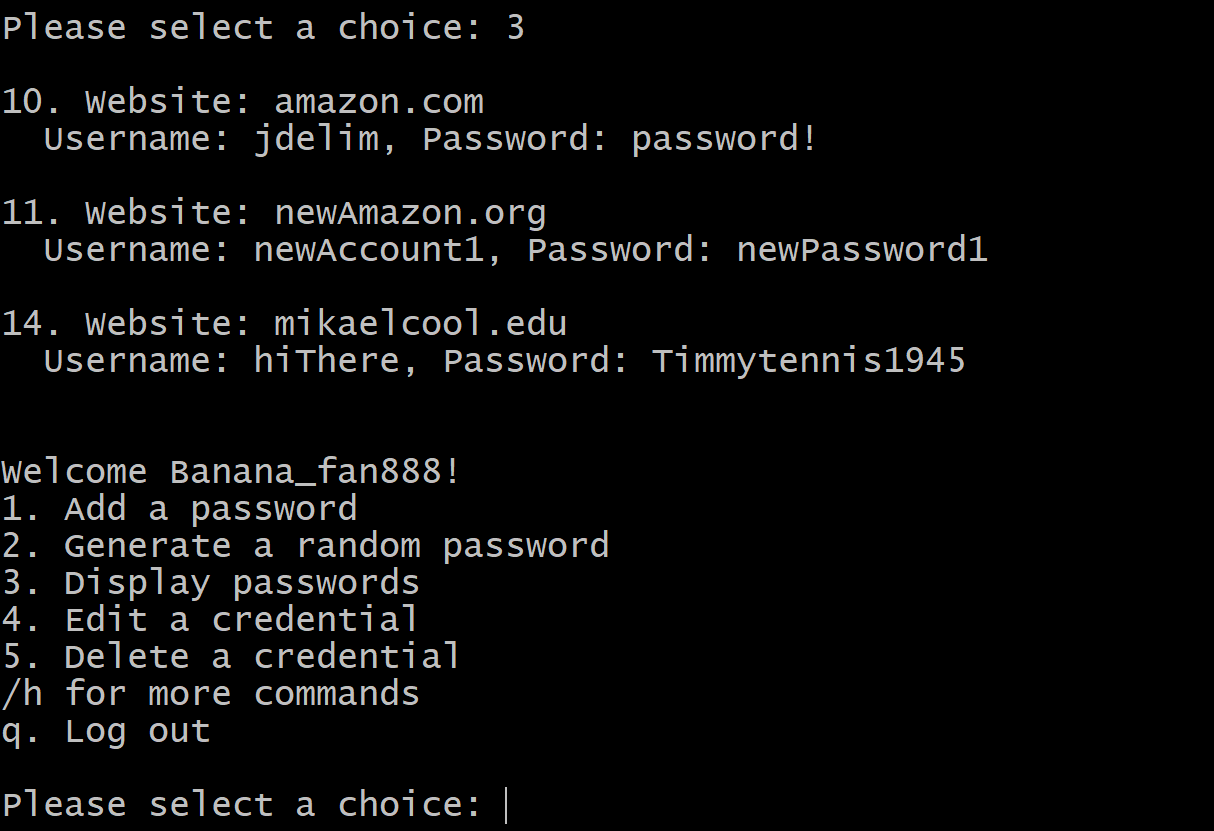
\includegraphics[width=0.5\textwidth]{evalResults.PNG}
    \caption{Displaying plaintext passwords in CLI.}
    \label{DisplayPassCLI}
\end{figure}

\begin{figure}[h]
    \centering
    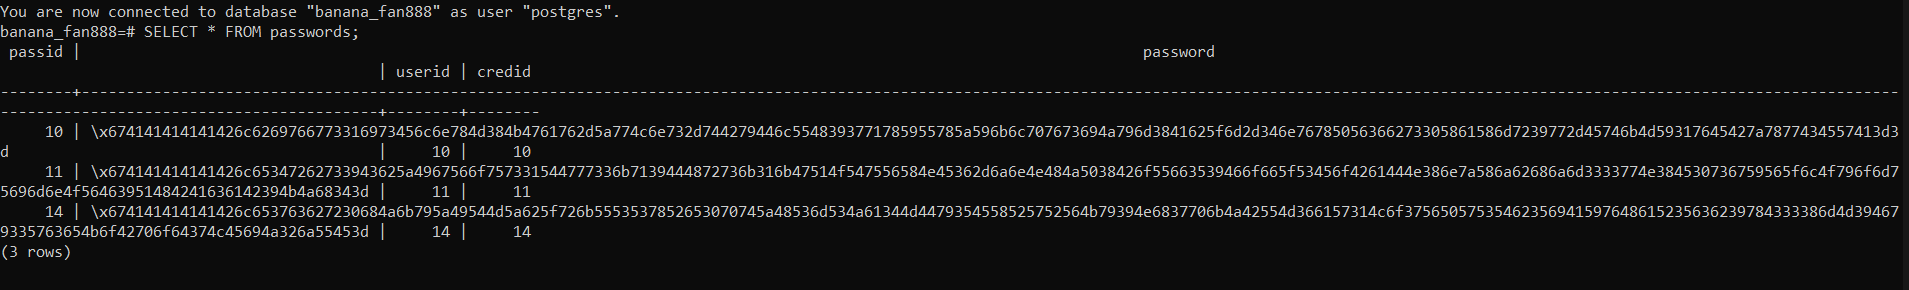
\includegraphics[width=0.5\textwidth]{PSQLResults.PNG}
    \caption{Showing the encrypted passwords in PostgreSQL.}
    \label{PSQLResults}
\end{figure}

\paragraph{}
Furthermore, while users expressed positive feedback over the general functionality of the password manager, one of the main points of critique were the lack of features that would give them a better sense of security and usability. For instance, two-factor authentication, having the ability to sync passwords across devices, and having more customizability in regards to grouping certain credentials together. This is highly important feedback as I've learned that just understanding about password managers and using one is not convincing enough for people to understand the importance of password managers. Rather, a combination of a lot of convenient and customizable features to make it easier for the user to implement in their day-to-day online activities is a big draw for people to use password managers as well as understanding the security behind it. In fact, one of the leading reasons why people do not use password managers is because of a lack of trust\cite{Yee_Editor_2022}.

\section{Ethical Considerations}
% Are there any ethical concerns that might arise from your project?
% You might think about whether your project perpetuates societal inequity (or could be used by others to do so), whether the data/platforms you are using is collected with informed consent and free of bias, and whether you might be subject to technological solutionism instead of working support/better the public infrastructure.
% Include a discussion of how you plan to mitigate these issues in your project.
\subsection{Brief Introduction}
Because my project is a password manager and handling user data, I must consider that the data I am working with is sensitive despite the fact that it might not be a real product. This is because this project is not only an implementation of cryptography, but also practice on how to appropriately manage sensitive customer data (usernames and passwords). When it comes to password managers, the main ethical concerns that arise have to do with trust and security between the user and the developer. More specifically, can users trust that the developers behind the program will not use their information maliciously, and if a third-party attacker manages to gain unwarranted access in any way, how transparent will the developer/organization be with its users? My project will take into account the ethical responsibility of the developer in handling user data, being transparent with the code, and how communication plays a role in ethical responsibility.

\subsection{Ethical Responsibility of the Developer}
First, the initial concern many people have when it comes to password managers is if the developers behind it have access to their sensitive information. To alleviate this concern, I plan on adopting a ``zero-knowledge" protocol password manager structure where only the user can have access to their unencrypted data. Zero knowledge protocols are cryptographic protocols ``which do not reveal the information or secret itself during the protocol, or to any eavesdropper" \cite{aronsson1995zero}. However, a potential downside to this is that if the user ever forgets their master password, they will have no way to recover their account since only they have access to their account. Furthermore, another concern is that some password managers have been known to gather data on users to help it ``improve and optimize the product" \cite{porter_2021}. While they claim not to be sending identifying or sensitive customer information, it is usually seen as bad practice especially for a service that is so critical on protecting customer information.
\paragraph{}
When it comes to algorithms, it is also the responsibility of the developer to choose and/or create an algorithm that is as fair and unbiased as they can make it. This is because biased algorithms can have disastrous effects such as systematic discrimination against black people in the US healthcare system \cite{ledford2019millions}. While a biased algorithm will not always have such a large wide-scale impact in the given example, there may be a subset of people negatively affected. In my password manager, there is not really a way for a cryptographic algorithm to prioritize a certain user based on their ethnic group, race, or other personal identifiers. However, when it comes to user interface, they ``are likely to be particularly prone to emergent bias because interfaces by design seek to reflect the capacities, character, and habits of prospective users" \cite{friedman1996bias}. I recognize that having a command-line interface may be more difficult for the average user compared to someone with a computer science background, so I will try to alleviate this concern by implementing easy navigability through simple commands.
\subsection{Transparency}
Additionally, there is also the ethical responsibility to be as transparent as possible on how the system is handling customer data without sacrificing security. This is where Kerckhoff's Principle, a basic cryptography principle, comes into play which states that the security of the system depends on everything but the key being publicly known. Essentially, no detail of the implementation of my cryptographic system will be kept hidden from the user except for the keys involved. This accomplishes two things: gives transparency to how their data is being used while maintaining security and allows others to look for any potential vulnerabilities in the system which can be remedied faster\cite{mrdovic2008kerckhoffs}.
\paragraph{}
To add, part of being transparent and adhering to Kerckhoff's Principle is keeping my project open-source. This means publicly hosting the repository on GitHub, allowing anyone to see it. This means that I can potentially show my code to coding/cryptography communities such as on Reddit or Discord or cryptographic professionals and experts to receive feedback on the overall architecture of my code as well as any potential security vulnerabilities if I ever wanted to in the future. Having a password manager being open to constant testing by others in the online community can only help to aid the overall security of it.
\subsection{Communication}
Communication and transparency go hand in hand when it comes to handling sensitive customer information. Take, for instance, the recent LastPass leak incident where they hid the fact that encrypted customer vaults had been taken for months \cite{clark_2022}. Many users have lost faith and trust in LastPass, not because of a weak system structure or algorithm, but its lack of communication to its users. It is not a question of \emph{if} a password manager will be compromised, but \emph{when}, and when it happens it is the ethical responsibility of the developers/organization to let its users know.
\paragraph{}
To expand on the LastPass incident, it was not just a failure of communication, but also the failure of lying about having a ``zero-knowledge" architecture and other bad cryptographic practices \cite{clark_2022}. Not only did they fail to communicate with their users, but the lack of an open-source architecture meant that there was no way for users to ensure that LastPass was truly following a ``zero-knowledge" policy. As a result, LastPass's weak cryptographic practices went under the radar, putting user information at risk. Furthermore, LastPass has deflected some of the blame on the users themselves, saying that as long as ``you use its defaults for password length and strengthening and haven't reused it on another site", it would be impossible for hackers to crack it \cite{clark_2022}. In other words, if customers' passwords were decrypted, it was because the customers didn't follow the best practices. 

\section{Future Work and Conclusion}
In terms of future work, there is a lot to be done on the front-end and back-end. For the front-end, it could be developed into some sort of web-app where user interaction will be much more fluid and smooth. Users will be able to click around, go back and forth easily between pages, use multiple features, and much more. Many password managers already do this so there is much to take inspiration from.  For the back-end, it is possible to migrate the database to the cloud so it can be synced across multiple computers. Of course, there will be other security implications to take into account when storing encrypted data remotely compared to just locally. 
\paragraph{}
Overall, this password manager project has not only helped me learn more about encryption, database management, and user interface, but also the overall process of developing an application/program. This involves receiving feedback from peers (or coworkers), interacting with potential users and receiving feedback, and lots of constant testing. Coming up with my own cryptographic scheme and designing the database were probably the most challenging aspects of this project, and then having to make them interact with each other was even more difficult. However, diagramming, brainstorming, and drawing out the outline of the project was extremely helpful in preventing future headaches as I could break it down into smaller manageable chunks once I knew the overall scope of the project.

\section{Code Documentation}

% This section will demonstrate that you have thought through the basics of how your code will work. You should include a diagram of the overall data flow of your program, including what the inputs and outputs of each component will be, and how they will be represented.

There are two main parts of my password manager: account creation and account login.

\paragraph{}
In the account creation flow\ref{AccountCreation}, the user inputs a valid username and master password. An RKEY and salt value is generated alongside this which has no relation to the user's inputs. The master password goes through a key derivation function, outputs a DKEY, enters an encryption function with the RKEY and salt values, and outputs an EKEY which is stored in the ekeys database. The username and salt is also stored alongside with the EKEY. The RKEY is used to encrypt user data.

\begin{figure}[h]
    \centering
    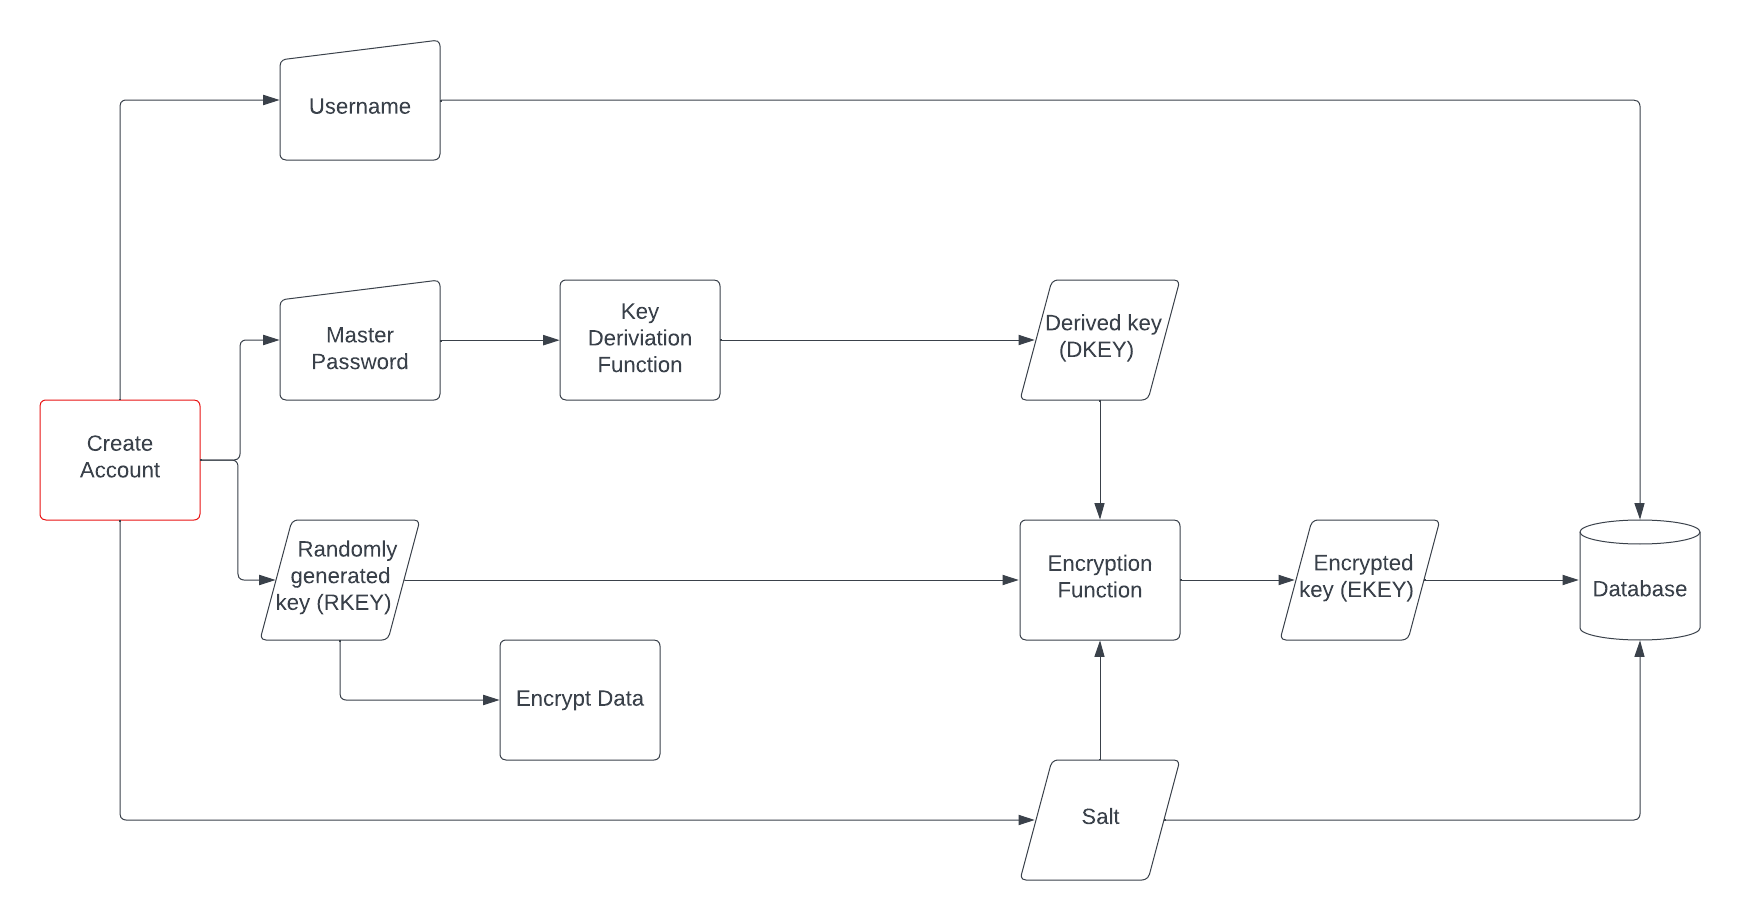
\includegraphics[width=0.5\textwidth]{Account Creation Flow.png}
    \caption{Account creation flow diagram.}
    \label{AccountCreation}
\end{figure}

\paragraph{}
In the login flow, the user enters a username and master password\ref{LoginFlow}. The corresponding username is found in the ekeys database and its corresponding EKEY and salt values are retrieved. The master password, along with the retrieved salt value, is passed through the key derivation function which outputs a DKEY. This DKEY and the retrieved EKEY is passed through the key decryption function and outputs an RKEY which is used to decrypt user data. If the user enters an incorrect master password, the incorrect RKEY (or no RKEY) will be generated and unable to decrypt the data.

\begin{figure}[h]
    \centering
    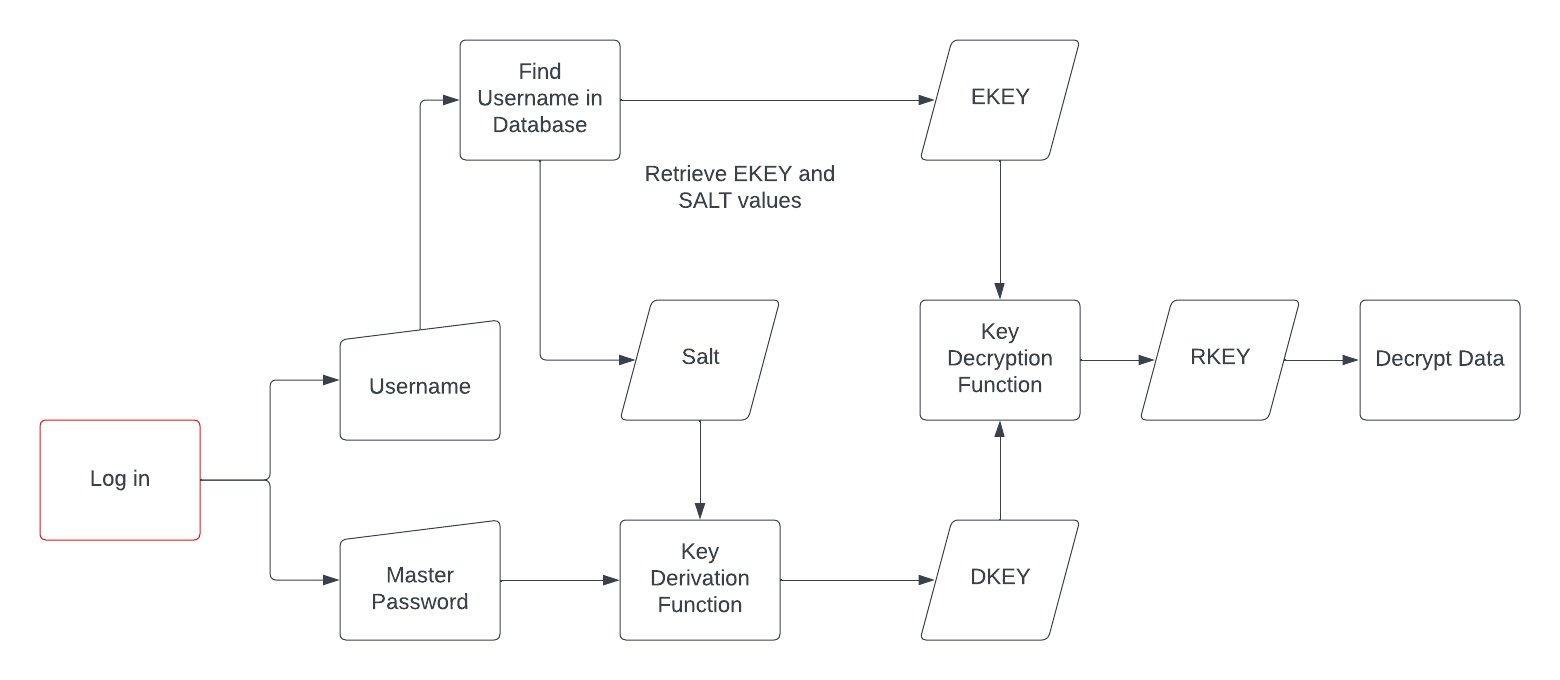
\includegraphics[width=0.5\textwidth]{Login Flow.png}
    \caption{Login flow diagram.}
    \label{LoginFlow}
\end{figure}

\section{Appendices}

\subsection{Replication Instructions}
First, ensure that you have the latest version of PostgreSQL and Python installed. The PostgreSQL version used here was version 16 for Windows. After installing PostgreSQL, make sure to remember the password you entered during installation and the name of the default database (most likely it is called 'postgres'). Also, look at the REQUIREMENTS.txt file to find the list of packages to install for Python. After installing PostgreSQL and the necessary packages, change the name of the database parameter value in database.ini to the default database name. Double check to see if the other parameter values are correct with the ones installed in your PostgreSQL version. Now that we have everything set-up, run intialize.py. If this doesn't work, double check the values in database.ini (particularly the name of the database and the password!). After running initialize.py, change the name of the database in database.ini back to `ekeys'. Finally, run main.py and enjoy the password manager!

\subsection{Code Architecture Overview}
The majority of the code can be found in database.py, encryption.py, and main.py. I tried to separate the code into different .py files according to what role it will play in the overall password manager. Database.py has to do with any and all interactions involving the PostgreSQL database, encryption.py is essentially the implementation of the encryption structure mentioned earlier with the EKEYs, RKEYs, and DKEYs, and main.py is the overall password manager program utilizing functions from the different .py files. Other smaller files include config.py which has to do with interaction between database connection and database.ini, education.py which simply contains a CommandHandler with print statements and password strength checker functions, initialize.py to set-up the database for first-time execution of the program, passwordgeneration.py, and ui.py. Ui.py was initially intended to contain the functions for the account creation and login flows, but, due to time constraints and errors, was mostly used for testing. Once those functions in ui.py are eventually completed and working, main.py will be more organized and look a lot cleaner.
\paragraph{}
First, database.py contains functions which have to do with establishing connection with the database, running queries on the database involving creating, reading, updating, and deleting rows of information, creation of users, databases, and tables, and displaying information from the database. There aren't really any algorithms at play here, however it does utilize encryption and decryption functions from encryption.py to insert encrypted information into databases and retrieve the plain-text from those encrypted data.
\paragraph{}
Next, encryption.py contains functions which generate the DKEY, EKEY, and RKEY as well as functions that encrypt and decrypt data using the RKEY. The function that generates the DKEY uses the PBKDF2 algorithm to derive a key from a master password, salt included. Generating the RKEY is pretty straightforward, using the Fernet.generate\_key() method. Encrypting and decrypting the symmetric key (RKEY) are both similar functions with different parameters. The encrypting function takes in the RKEY and DKEY, passes them through the Fernet cipher, and outputs the EKEY. The decrypting function takes in the EKEY and DKEY, passes them through the Fernet cipher, and outputs the RKEY. The encrypt and decrypt data functions are also in a similar manner, where the former takes in data and the RKEY, passes it through the Fernet cipher, and outputs the encrypted data. The latter takes in the encrypted data and RKEY, passes it through the Fernet cipher, and outputs the decrypted data.
\paragraph{}
Finally, main.py puts it password manager all together. In the main menu, categorized by the first while loop, contains the account creation and login flow which can be selected via entering an integer and being passed through elif statements. When an account is created, that user's username, EKEY, and salt values are stored in the ekeys table. In order to leave the main menu and gain access to their account, the user must successfully go through the login flow process by entering a correct username and master password combination. The second while loop represents the user having access to their account after logging in where they are then given the option to add passwords, generate a random password, display passwords, edit, and delete passwords. These have a similar structure to the main menu while loop where they enter an integer and it is passed through elif statements. 


\printbibliography

\end{document}
